\achapter{12}{Topological Spaces}\label{sec:top_spaces}


\vspace*{-17 pt}
\framebox{
\parbox{\dimexpr\linewidth-3\fboxsep-3\fboxrule}
{\begin{fqs}
\item What is a topology and what is a topological space?
\item What important properties do open sets have in relation to unions and intersections?
\item What is a basis for a topology? Why is a basis for a topology useful?
\item What is a neighborhood in a topological space?
\item What is an interior point and the interior of a set in a topological space?
\item What is the connection between the interior of a set and open sets in a topological space?
\end{fqs}}}

\vspace*{13 pt}

\csection{Introduction}

Many of the properties that we introduced in metric spaces (continuity, limit points, boundary) could be phrased in terms of the open sets in the space. With that in mind, we can broaden our concept of space by eliminating the metric and just defining the opens sets in the space. This produces what are called \emph{topological spaces}.


Recall that the open sets in a metric space satisfied certain properties, including that the arbitrary union of open sets is open and any finite intersection of opens sets is open. We will now take these properties as our axioms in defining topological spaces. 

\begin{definition} Let $X$ be a nonempty set. A set $\tau$\footnote{The symbol $\tau$ is the Greek lowercase letter tau.}
 of subsets of $X$ is said to a \textbf{topology}\index{topology} on $X$ if
\begin{enumerate}
\item $X$ and $\emptyset$ belong to $\tau$,
\item any union of sets in $\tau$ is a set in $\tau$, and
\item any finite intersection of sets in $\tau$ is a set in $\tau$.
\end{enumerate}
\end{definition}

A \emph{topological space}\index{topological space} is then any set on which a topology is defined. If $X$ is the space and $\tau$ a topology on $X$, we denote the topological space as $(X, \tau)$. The elements of $\tau$ are called the \emph{open sets}\index{open sets in a topological space} in the topological space. When the topology is clear from the context, we simple refer to $X$ as the topological space. Some examples are in order. 

\begin{pa} ~
\be
\item Suppose $X  = \{ a, b, c\}$. Is the set $\tau = \{a,b\}$ a topology on $X$? Justify your response. 

\item Suppose $X= \{a,b,c,d\}$. Is the collection of subsets consisting of $\tau = \{ \{a\}, \{b\}, \{a,b\} \}$ a topology on $X$? Justify your response. If not, what is the smallest collection of subsets of $X$ that need to be added to $\tau$ to make $\tau$ a topology on $X$? 

\item Suppose $X= \{a,b,c,d\}$. Is the collection of subsets consisting of 
\[\tau = \{\emptyset, \{a\}, \{b\}, \{d\}, \{a,b\}, \{a,d\}, X \}\]
a topology on $X$? Justify your response. If not, what is the smallest collection of subsets of $X$ that need to be added to $\tau$ to make $\tau$ a topology on $X$?.

\item Suppose $X= \{a,b,c,d\}$. Is the collection of subsets consisting of 
\[\tau = \{\emptyset, \{a\}, \{b\}, \{c\}, \{d\}, \{a,b\}, \{a,c\}, \{a,d\}, \{b, d\}, \{c,d\}, X \}\]
a topology on $X$? Justify your response. If not, what is the smallest collection of subsets of $X$ that need to be added to $\tau$ to make $\tau$ a topology on $X$?

\item  Let $F$ be the collection of finite subsets of $\R$.  Let $\tau = \{\emptyset, \R\} \cup F$. First, list three members of $F$ and three sets that are not in $F$. Next, is $\tau$ a topology on $\R$? Justify your response.

\item Let $\tau = \{\emptyset, \R, \{0\} \}$. Is $\tau$ a topology on $\R$? Justify your response.

\item Let $X$ be a set and let $\tau = \{\emptyset, X\}$. Is $\tau$ a topology on $X$? Justify your response.

\item Let $X$ be a set and let $\tau$ be the collection of all subsets of $X$. Is $\tau$ a topology on $X$? Justify your response.

\ee

\end{pa}

\begin{comment}

\ActivitySolution

\be
\item  The answer is no. The elements of a topology must be subsets of the space $X$, not elements of $X$. 

\item  Since $\emptyset \notin \tau$, as given $\tau$ is not a topology on $X$. We need to add both $\emptyset$ and $X$ to $\tau$ in order for $\tau$ to be a topology on $X$. Once we do that, then $\tau$ is closed under intersections and unions, so $\tau =  \{\emptyset , \{a\}, \{b\}, \{a,b\} , X \}$ is a topology on $X$. 

\item  Notice that $\{b\} \cup \{d\}$ is not in $\tau$, so $\tau$ is not a topology on $X$. Since the single element sets $\{a\}$, $\{b\}$, and $\{d\}$ are all in $\tau$, any union of these sets will be in $\tau$. The fact that $c$ is no an element of any set in $\tau$ means that 
\[\tau = \{ \emptyset, \{a\}, \{b\}, \{d\}, \{a,b\}, \{a,d\}, \{b,d\}, \{a,b,d\}, X \}\]
is a topology on $X$.  

\item  Notice that $\{a,b\} \cup \{c\}$ is not in $\tau$, so $\tau$ is not a topology on $X$. Since the single element sets $\{a\}$, $\{b\}$, $\{c\}$, and $\{d\}$ are all in $\tau$, any union of these sets will be in $\tau$. This means that every subset of $X$ must be in $\tau$,so 
\[\tau = 2^X\]
is a topology on $X$. 

\item   The sets $\{1\}$, $\{1,2\}$, and $\{1,2,3\}$ are all in $F$, while the sets $(0,1)$, $\Z$, and $\Q$ are not in $F$. Notice that the sets $\{n\}$ for $n \in \Z$ are all in $F$, but $\bigcup_{n \in \Z} \{n\} = \Z$ is not in $F$. Thus, $\tau$ is not closed under arbitrary unions and $\tau$ is not a topology on $\R$. 

\item  By inspection we can see that $\tau$ is closed under unions and intersections, so $\tau$ is a topology on $\R$. 

\item  By inspection we can see that $\tau$ is closed under unions and intersections, so $\tau$ is a topology on $\R$. This topology is called the \emph{indiscrete} or \emph{trivial} topology. 

\item  By definition, $\tau$ is closed under unions and intersections, so $\tau$ is a topology on $X$. This topology is called the \emph{discrete} topology. 

\ee

\end{comment}

\csection{Examples of Topologies}

In our preview activity we saw several examples of topologies. Suppose $X$ is a nonempty set.
\begin{itemize}
\item The topology consisting of all subsets of $X$ is called the \emph{discrete topology}\index{topology!discrete}.
\item The topology $\{\emptyset, X\}$ is the \emph{indiscrete topology}\index{topology!indiscrete}. 
\item If $(X,d)$ is a metric space, then the collection consisting of unions of all open balls is a topology called the \emph{metric topology}\index{topology!metric}. This result tells us that every metric space is topological space under the metric topology. We will see later than not every topological space is a metric space. 
\end{itemize}
The discrete and indiscrete topologies are topologies that can be defined on any set and are often used to use to generate examples. Another topology that can be defined on any set is in the next activity. 

\begin{activity} \label{act:TS_limits} Let $X$ be any set and let $\tau_{FC}$ consist of the empty set along with all subsets $O$ of $X$ such that $X \setminus O$ is finite. 
\ba
\item Prove that $\tau_{FC}$ is a topology on $X$. (The topology $\tau_{FC}$ is called the \emph{finite complement topology}\index{topology!finite complement} or the \emph{cofinite topology}\index{topology!cofinite}. 

\item Explain why $\tau_{FC}$ is the discrete topology when $X$ is finite.

\ea

\end{activity}

\begin{comment}

\ActivitySolution 

\ba

\item By definition, $\emptyset \in \tau_{FC}$. Since $X \setminus X = \emptyset$ is finite, $X \in \tau_{FC}$. Let $\{O_{\alpha}\}$ be a collection of open sets in $X$ for $\alpha$ in an indexing set $I$. Since $X \setminus O_{\alpha}$ is finite for each $\alpha \in I$, we have that 
\[X \setminus \bigcup_{\alpha \in I} O_{\alpha} = \bigcap_{\alpha \in I} (X \setminus O_{\alpha}) \subseteq (X \setminus O_{\beta}\]
for any $\beta \in I$ is a finite set. Thus, $\bigcup_{\alpha \in I} O_{\alpha} \in \tau_{FC}$. 

Now suppose that $I$ is finite. Then
\[X \setminus \bigcap_{\alpha \in I} O_{\alpha} = \bigcup_{\alpha \in I} (X \setminus O_{\alpha})\]
is a finite union of finite sets and so is finite. Thus, $\bigcap_{\alpha \in I} O_{\alpha} \in \tau_{FC}$. We conclude that $\tau_{FC}$ is a topology. 

\item Suppose $X$ is finite. Then $X \setminus O$ is finite for every subset $O$ of $X$. Thus, every subset of $X$ is open and so $\tau_{FC}$ is the discrete topology.

\ea


\end{comment}

\csection{Bases for Topologies}

It can be difficult to completely describe the open sets in a topology. Instead, we can describe the topology using a collection of sets that generate the topology. For example, if $(X,d)$ is a metric space then the collection of open sets in $X$ forms a topology on $X$, called the \emph{metric}  topology. We also saw that in a metric space, every open set in $X$ is a union of open balls. For that reason we called the collection of open balls a \emph{basis} for the open sets in $X$. We can do the same thing in any topological space. As a non-trivial example, an interesting topology defined on the positive integers is due to S.W. Golomb.  One can use this topology to prove that there are infinitely many primes. This topology also makes the positive integers into a connected Hausdorff space (more on these concepts later). The Golomb topology is defined as follows. If $a$ and $b$ are coprime integers in $\Z^+$ (that is, $a$ and $b$ have no common positive factors other than 1 so that the greatest common divisor of $a$ and $b$ is $1$), let 
\[B_{a,b} = \{a+bn \mid n \geq 0\}.\]
The collection of sets $B_{a,b}$ is a basis for the Golomb topology, and the topological space $(\Z^+, \tau)$ is called the \emph{Golomb space}\index{Golomb space}. It is an exercise in number theory to prove that the sets $B_{a,b}$ form a basis for a topology, so we will not go into the details. 

\begin{activity} \label{act:top_basis} Let $X = \{a,b,c,d\}$ and let $\tau = \{\emptyset, \{a\}, \{b\}, \{a,b\}, \{c,d\}, \{a,c,d\}, \{b,c,d\},X)$. You may assume that $\tau$ is a topology on $X$. Explain why any nonempty open set in the topological space $(X, \tau)$ can be written in terms of arbitrary unions and finite intersections of $\{a\}$, $\{b\}$, and $\{c,d\}$. 

\end{activity}

\begin{comment}

\ActivitySolution By exhaustively looking at every nonempty open set we can see that 
\begin{align*}
\{a\} &= \{a\} \\
\{b\} &= \{b\} \\
\{a,b\} &= \{a\} \cup \{b\} \\
\{c,d\} &= \{c,d\} \\
\{a,c,d\} &= \{a\} \cup \{c,d\} \\
X &=  \{a\} \cup \{b\} \cup \{c,d\}.
\end{align*}

\end{comment}

Activity \ref{act:top_basis} shows that, just like the open balls in a metric space, a topology can have a collection of subsets whose unions make up all of the open sets in the topology. We do need to take a little care, though. A basis will generate the collection of open sets for a topology, so the basis sets we start with should themselves be open sets. In addition, every element in the topological space should be an element of one of the basis sets, and since the basis elements are to produce all of the open sets in the topology, every set in the topology (except the empty set) should be a union of sets in a basis. It also must be the case that we can ensure that any finite intersection of sets in the topology remains a set in the topology when we write the sets in the topology in terms of the sets in a basis. To make the last two conditions happen, we will see that it is enough to insist that for any point in the intersection of basis elements, there is another basis element in that intersection that contains the point. This is summarized in Theorem \ref{thm:Basis}.  

\begin{theorem} \label{thm:Basis} Let $X$ be a set and let $\B$ be a collection of subsets of $X$ such that 
\begin{enumerate}
\item For each $x \in X$, there is a set in $\B$ that contains $x$.
\item If $x \in X$ is an element of $B_1 \cap B_2$ for some $B_1, B_2 \in \B$, then there is a set $B_3 \in \B$ such that $x \in B_3 \subseteq B_1 \cap B_2$. 
\end{enumerate}
Then the set $\tau$ that consists of the empty set and unions of elements of $\B$ is a topology on $X$.  
\end{theorem}

Before we prove Theorem \ref{thm:Basis}, we will need to know one fact about the set $\B$. 

\begin{activity} \label{act:Basis} Let $X$ be a set and $\B$ a collection of subsets of $X$ such that
\begin{enumerate}
\item For each $x \in X$, there is a set in $\B$ that contains $x$.
\item If $x \in X$ is an element of $B_1 \cap B_2$ for some $B_1, B_2 \in \B$, then there is a set $B_3 \in \B$ such that $x \in B_3 \subseteq B_1 \cap B_2$. 
\end{enumerate}
Let $B_1$, $B_2$, $\ldots$, $B_n$ be in $\B$. Our goal in this activity is to extend property 2 and show that if $x \in \bigcap_{1 \leq k \leq n} B_k$, then there is a set $B \in \B$ such that $x \in B$ and $B \subseteq \bigcap_{1 \leq k \leq n} B_k$. 
\ba
\item Since the statement we want to prove depends on a positive integer $n$, we will use mathematical induction. Explain why the $n=1$ and $n=2$ cases are true.

\item What is the inductive hypothesis and what do we want to prove in the inductive step? 

\item Use the inductive hypothesis and condition 2 to complete the proof of the following lemma.

\begin{lemma} \label{lem:Basis} Let $X$ be a set and $\B$ a collection of subsets of $X$ such that
\begin{enumerate}
\item For each $x \in X$, there is a set in $\B$ that contains $x$.
\item If $x \in X$ is an element of $B_1 \cap B_2$ for some $B_1, B_2 \in \B$, then there is a set $B_3 \in \B$ such that $x \in B_3 \subseteq B_1 \cap B_2$. 
\end{enumerate}
Let $B_1$, $B_2$, $\ldots$, $B_n$ be in $\B$. If $x \in \bigcap_{1 \leq k \leq n} B_k$, then there is a set $B \in \B$ such that $x \in B$ and $B \subseteq \bigcap_{1 \leq k \leq n} B_k$. 
\end{lemma}

\ea

\end{activity}

\begin{comment}

\ActivitySolution

\ba
\item The $n=1$ case is true by property (1) of $\B$, since a set $B_x$ that contains $x$ is a subset of itself. The $n=2$ case is the assumption (2).  

\item For the inductive hypothesis we assume that for some integer $n \geq 1$, if $B_1$, $B_2$, $\ldots$, $B_n$ are in $\B$ and $x \in \bigcap_{1 \leq k \leq n} B_k$, then there is a set $B \in \B$ such that $x \in B$ and $B \subseteq \bigcap_{1 \leq k \leq n} B_k$. We want to prove that if we have sets $B_1$, $B_2$, $\ldots$, $B_n$, $B_{n+1}$ in $\B$ and $x \in \bigcap_{1 \leq k \leq n+1} B_k$, then there is a set $B \in \B$ such that $x \in B$ and $B \subseteq \bigcap_{1 \leq k \leq n+1} B_k$.

\item  Assume the lemma is true for some $n \in \Z^+$ and assume that we have sets $B_1$, $B_2$, $\ldots$, $B_n$, $B_{n+1}$ in $\B$ and $x \in \bigcap_{1 \leq k \leq n+1} B_k$. Then $x \in \bigcap_{1 \leq k \leq n} B_k$, so by our induction hypothesis there is a set $B' \in \B$ with $x \in B'$ and $B' \subseteq \bigcap_{1 \leq k \leq n} B_k$. Now $x \in B' \cap B_{n+1}$, so condition 2 implies that there is a set $B \in \B$ with $x \in B$ and $B \subseteq B' \cap B_{n+1} \subseteq \bigcap_{1 \leq k \leq n+1} B_k$. This completes our proof.

\ea

\end{comment}

Now we can prove Theorem \ref{thm:Basis}.

\begin{proof}[Proof of Theorem  \ref{thm:Basis}] Let $X$ be a topological space, and let $\B$ and $\tau$ satisfy the given conditions. By definition, $\emptyset \in \tau$. For each $x \in X$ there is a set $B_x \in \B$ such that $x \in B_x$. Then $X = \bigcup_{x \in X} B_x$, and $X \in \tau$. To complete our proof that $\tau$ is a topology on $X$, we need to demonstrate that $\tau$ is closed under arbitrary unions and finite intersections. We first consider unions. Let $\{U_{\alpha}\}$ be a collection of sets in $\tau$ for $\alpha$ in some indexing set $I$. By definition, each $U_{\alpha}$ is empty or is a union of elements of $\B$. So either $U = \bigcup_{\alpha \in I} U_{\alpha}$ is empty, or is a union of sets in $\B$. Thus, $U \in \tau$ and $\tau$ is closed under arbitrary unions. 

Now we show that $\tau$ is closed under finite intersections. Let $n$ be a positive integer and let $\{U_{k}\}$ a collection of sets in $\tau$ for $1 \leq k \leq n$. Let $U = U_1 \cap U_2 \cap \cdots \cap U_n$. If $U_k = \emptyset$ for any $k$, then $U = \emptyset$ is in $\tau$. So suppose that $U_k \neq \emptyset$ for each $k$ between $1$ and $n$. Let $x \in U$. Then $x \in U_k$ for each $k$. For every $m$ between $1$ and $n$, the fact that $U_m$ is a union of elements in $\B$ implies that there exists $B_m \subseteq U_m$ with $x \in B_m$. Thus, $x \in \bigcap_{1 \leq m \leq n} B_m$. 

Lemma \ref{lem:Basis} shows that there is a set $B_x \in \B$ such that $x \in B_x$ and $B_x \subseteq \bigcap_{1 \leq m \leq n} B_m \subseteq \bigcap_{1 \leq m \leq n} U_m = U$. Since $x$ is an arbitrary element of $U$, we must have $U \subseteq \bigcup_{x \in U} B_x$. But each $B_x$ is subset of $U$, so $\bigcup_{x \in U} B_x \subseteq U$. It follows that 
\[U = \bigcup_{x \in U} B_x\]
and $U \in \tau$. Therefore, $ \tau$ is a topology on $X$.
\end{proof}

Any collection $\B$ of sets as given in Theorem \ref{thm:Basis} is given a special name.

\begin{definition} \label{def:basis_topology} Let $X$ be a set. A set $\B$ is a \textbf{basis for a topology}\index{basis!for a topology} (or just a \textbf{basis}) on $X$ if 
\begin{enumerate}
\item For each $x \in X$, there is a set in $\B$ that contains $x$.
\item If $x \in X$ is an element of $B_1 \cap B_2$ for some $B_1, B_2 \in \B$, then there is a set $B_3 \in \B$ such that $x \in B_3 \subseteq B_1 \cap B_2$. 
\end{enumerate}
\end{definition}

 The elements of a basis $\B$ are called \emph{basis elements}\index{basis!elements} or the \emph{basic open sets}\index{basic open set}. A basis for a topology on a set $X$ defines a topology on $X$ as shown in Theorem \ref{thm:Basis}.
 
 Note that because of property (1) of Definition \ref{def:basis_topology}, the union of the sets in the basis must contain $X$. In other words, the sets in a basis cover the space. The second property ensures that if a point is in the intersection of two basic open sets, then there is a smaller basic open set that contains $x$. 

\begin{definition} Let $\B$ be a basis for a topology on a set $X$. The \textbf{topology $\tau$ generated by $\B$}\index{topology generated by a basis} contains the empty set and all arbitrary unions of basis elements.
\end{definition}

When the topology for a space $X$ is clear from the context, we also call a basis for the topology a basis for $X$. 

\begin{activity} ~
\ba
\item Let $X=\{a,b,c,d,e,f\}$ and $\tau= \{\emptyset, \{a\}, \{c,d\},\{a,c,d\}, \{b,c,d,e,f\}, X \}$. 
	\begin{enumerate}[i.]
	\item Is the set 
	\[\mathcal{B}  = \{\{a\},\{a,c,d\} \}\] 
a basis for $\tau$? If not, add the smallest number of sets that you can to $\mathcal{B}$ to make a basis for this topology.

	\item Is the set 
\[\mathcal{B}  = \{\{a\},\{c,d\},\{b,c,d,e,f\} \}\] 
a basis for $\tau$? If not, add the smallest number of sets that you can to $\mathcal{B}$ to make a basis for this topology.

	\end{enumerate}

\item Let $X=\{a,b,c\}$ and let $X$ have the discrete topology (the topology consisting of all subsets of $X$). Is $\mathcal{B}  = \{\{a\},\{c\},\{a,b\},\{b,c\} \}$ a basis for $\tau$ in the the discrete topology? If not, add the smallest number of sets that you can to $\mathcal{B}$ to make a basis for this topology.

\item Find a basis for the discrete topology on any set $X$.

\ea

\end{activity}

\begin{comment}

\ActivitySolution

\ba
\item 
	\begin{enumerate}[i.]
	\item Since there is no set in $\mathcal{B}$ that contains the element $b$, the set $\mathcal{B}$ is not a basis for the topology $\tau$. Since every set in $\mathcal{B}$ must be an open set, and every set in $\tau$ has to be a union of sets in $\mathcal{B}$, we need add the open sets $\{c,d\}$ and $\{b,c,d,e,f\}$ to $\mathcal{B}$ to make a basis for the topology.
	
	\item Since
\begin{align*}
\{a\} &= \{a\} \\
\{c,d\} &= \{c,d\} \\
\{a,c,d\} &= \{a\} \cup \{c,d\} \\
\{b,c,d,e,f\} &= \{b,c,d,e,f\}
X &=  \{a\} \cup\{b,c,d,e,f\},
\end{align*}
we conclude that $\mathcal{B}$ is a basis for $\tau$

	\end{enumerate}
	
\item The set $\mathcal{B}$ is not a basis for $\tau$ because $\{b\}$ is not a union of sets in $\mathcal{B}$. If we add $\{b\}$ to $\mathcal{B}$, then we have all of the single point sets. Every subset of $X$ can be made of a union of single point sets, which then produces a basis for $\tau$. 

\item Since every single point set is open, our basis has to include all single point sets. But every subset of $X$ can be made of a union of single point sets, which explains why the collection of single points sets is a basis for $\tau$. 

\ea

\end{comment}

\csection{Metric Spaces and Topological Spaces}

Every metric space is a topological space, where the topology is the collection of open sets defined by the metric. This topology is called the \emph{metric topology}\index{topology!metric}. A natural question to ask is whether every topological space is a metric space. That is, given a topological space, can we define a metric on the space so that the open sets are exactly the sets in the topology? For example, any space with the discrete topology is a metric space with the discrete metric. 

\begin{activity} Let $X = \{a,b,c,e\}$ and $\tau = \{\emptyset, \{a\}, \{b\}, \{a,b\}, X \}$. Explain why there cannot be a  metric $d : X \times X \to \R$ so that the open sets in the metric topology are the sets in $\tau$. (Hint: Assume that such a metric exists and consider the open balls centered at $c$.)  

\end{activity}

\begin{comment}

\ActivitySolution Assume such a metric $d$ exists. Let $r = d(a,c)$. Then $B(c,r)$ is an open set containing $c$. The only such open set is $X$, but $d(a,c) < r$ implies that $a \notin B(c,r)$. This contradiction shows that no such metric exists.  

\end{comment}

We conclude that every metric space is a topological space, but not every topological space is a metric space. The topological spaces that can be realized as metric spaces are called \emph{metrizable}\index{metrizable topological space}. 

\csection{Neighborhoods in Topological Spaces}

Recall that we defined a neighborhood of a point $a$ in a metric space to be a subset of the space that contains an open ball centered at $X$. Every open ball is an open set, so we can extend the idea of neighborhood to topological spaces.

\begin{definition} Let $(X, \tau)$ be a topological space, and let $a \in X$. A subset $N$ of $X$ is a \textbf{neighborhood}\index{neighborhood in a topological space} of $a$ if $N$ contains an open set that contains $a$. 
\end{definition}

Let's look at some examples.

\begin{activity} Let $X = \{a,b,c,d\}$ and let $\tau = \{\emptyset, \{a\}, \{b\}, \{a,b\}, X \}$. 
\ba
\item Find all of the neighborhoods of the point $a$. 

\item Find all of the neighborhoods of the point $c$.

\ea

\end{activity}

\begin{comment}

\ActivitySolution

\ba
\item The open sets that contain $a$ are $\{a\}$, $\{a,b\}$, and $X$. So the neighborhoods of $a$ are the subsets of $X$ that contain these open sets, or 
\[\{a\}, \ \{a,b\}, \ \{a,c\}, \ \{a,d\}, \ \{a,b,c\}, \ \{a,b,d\}, \ \text{ and } \ X.\] 

\item The only open set containing $c$ is $X$, so $X$ is the only neighborhood of $c$. 

\ea

\end{comment}

In metric spaces, an open set was a neighborhood of each of its points. This is also true in topological spaces.

\begin{theorem} Let $(X, \tau)$ be a topological space. A subset $O$ of $X$ is open if and only if $O$ is a neighborhood of each of its points.
\end{theorem}

\begin{proof} Let $(X, \tau)$ be a topological space, and let $O$ be a subset of $X$. First we demonstrate that if $O$ is open, then $O$ is a neighborhood of each of its points. Assume that $O$ is an open set, and let $a \in O$. Then $O$ contains the open set $O$ that contains $a$, so $O$ is a neighborhood of $a$.

The reverse containment is the subject of the next activity.
\end{proof}

\begin{activity} Let $(X, \tau)$ be a topological space. Let $O$ be a subset of $X$. Assume $O$ is a neighborhood of each of its points. 
\ba
\item  What do we need to do to show that $O$ is an open set?

\item Let $a \in O$. Why must there exist an open set $O_a$ such that $a \in O_a \subseteq O$?

\item Complete the proof that $O$ is an open set. 

\ea

\end{activity}

\begin{comment}

\ActivitySolution

\ba
\item  To prove that $O$ is open, we can write $O$ as a union of open sets.

\item Let $a \in O$. Since $O$ is a neighborhood of $a$, there exists an open set $O_a$ such that $a \in O_a \subseteq O$.

\item We will show that 
\[\bigcup_{a \in O} O_a = O.\]
Since any union of open sets is an open set, this will verify that $O$ is an open set. Since $O_a \subseteq O$ for each $a \in O$, it follows that $\ds \bigcup_{a \in O} O_a \subseteq O$. Now let $x \in O$. Then $x \in O_x \subseteq \bigcup_{a \in O} O_a$ and $O \subseteq \bigcup_{a \in O} O_a$. 

\ea

\end{comment}

\csection{The Interior of a Set in a Topological Space}

We have seen that topologies define the open sets in a topological space. As in metric spaces, open sets can be characterized in terms of their interior points. We defined interior points in metric spaces in terms of neighborhoods -- the same holds true in topological spaces. 

\begin{definition} Let $A$ be a subset of a topological space $X$. A point $a \in A$ is an \textbf{interior point}\index{interior point} of $A$ if $A$ is a neighborhood of $a$.
\end{definition}

Remember that a set is a neighborhood of a point if the set contains an open set that contains the point. By definition, every open set is a neighborhood of each of its points, so every point of an open set $O$ is an interior point of $O$. Conversely, if every point of a set $O$ is an interior point, then $O$ is a neighborhood of each of its points and is open. This argument is summarized in the next theorem. 

\begin{theorem} Let $X$ be a topological space. A subset $O$ of $X$ is open if and only if every point of $O$ is an interior point of $O$. 
\end{theorem}

The collection of interior points in a set form a subset of that set, called the \emph{interior} of the set.

\begin{definition} The \textbf{interior} of a subset $A$ of a topological space $X$ is the set
\[\Int(A) = \{a \in A \mid a \text{ is an interior point of } A\}.\]
\end{definition}

\begin{activity} \label{act:interior} ~
\ba
\item Consider $(\R, \tau)$, where $\tau$ is the standard topology (by standard in this situation, we mean the metric topology determined by the Euclidean metric). Let $A=(-\infty,0)\cup (1,2]\cup \{3\}$ in $\R$. What is $\Int(A)$? What is the largest open subset of $\R$ contained in $A$?

\item Consider $(\R, \tau)$, where $\tau$ is the discrete topology (the one where all subsets are open). Let $A=(-\infty,0) \cup (1,2] \cup \{3\}$ in $\R$. What is $\Int(A)$? What is the largest open subset of $\R$ contained in $A$?

\item Consider $(\R, \tau)$, where $\tau$ is the finite complement topology (the one where the open sets are the empty set along with all subsets $O$ of $\R$ such that $\R \setminus O$ is finite). Let $A=(-\infty,0) \cup (1,2] \cup \{3\}$ in $\R$. What is $\Int(A)$? What is the largest open subset of $\R$ contained in $A$?

\item Let $X = \{a,b,c,d\}$ and let 
\[\tau = \{\emptyset, \{a\}, \{a,b\}, \{c\}, \{d\}, \{c,d\}, \{a,c,d\}, \{a,c\}, \{a,d\}, \{a,b,c\}, \{a,b,d\}, X\}.\]
Assume that $\tau$ is a topology on $X$. Let $A = \{b,c,d\}$. What is $\Int(A)$? What is the largest open subset of $X$ contained in $A$?

\ea

\end{activity}

\begin{comment}

\ActivitySolution

\ba
\item If $x \in (-\infty,0)$, then $B(x,|x|) \subseteq A$. If $x \in (1,2)$ and $r = \min\{x-1, 2-x\}$, then $B(x,r) \subseteq A$. So every point in $(-\infty,0) \cup (1,2)$ is an interior point of $A$. For any $\epsilon > 0$, the ball $B(2,\epsilon)$ contains points larger than $2$ and the ball $B(3,\epsilon)$ contains points larger than $3$. So neither $2$ nor $3$ is an interior point of $A$. This makes $\Int(A) = (-\infty,0) \cup (1,2)$. We also see that $\Int(A)$ is the largest open subset of $X$ contained in $A$.    

\item Since every subset of $\R$ is an open set, every set is a neighborhood of each of its points. That and the fact that $\Int(A) \subseteq A$ by definition allows us to conclude that $\Int(A) = A$. Since every set is open, the largest open set in $\R$ contained in $A$ is also $A$. 

\item Recall that a set $O$ is open in the finite complement topology if $\R \setminus O$ is finite. Since $\R \setminus A$ is not finite, no subset of $A$ is open and so no subset of $A$ can be a neighborhood of each of its points. It follows that $\Int(A) = \emptyset$. By the same reasoning, $A$ contains no open subset of $\R$, so the largest open subset of $\R$ contained in $A$ is $\emptyset$. 

\item Since $\{c\} \subseteq A$ and $\{d\} \subseteq A$, we see that $c$ and $d$ are interior points of $A$. However, there is no open subset of $A$ that contains $b$, so $b$ is not an interior point of $A$. It follows that $\Int(A) = \{c,d\}$, which is also the largest open subset of $X$ contained in $A$. 

\ea

\end{comment}


One might expect that the interior of a set is an open set, as it was in metric spaces. This is true, but we can say even more. In Activity \ref{act:interior} we saw that in our examples that $\Int(A)$ was the largest open subset of $X$ contained in $A$. That this is always true is the subject of the next theorem. 

\begin{theorem} \label{thm:Interior} Let $(X,d)$ be a topological space, and let $A$ be a subset of $X$. The interior of $A$ is the largest open subset of $X$ contained in $A$.  
\end{theorem}

\begin{proof} Let $X$ be a topological space, and let $A$ be a subset of $X$. We need to prove that $\Int(A)$ is an open set in $X$, and that $\Int(A)$ is the largest open subset of $X$ contained in $A$. First we demonstrate that $\Int(A)$ is an open set. Let $a \in \Int(A)$. Then $a$ is an interior point of $A$, so $A$ is a neighborhood of $a$. This implies that there exists an open set $O$ containing $a$ so that $O \subseteq A$. But $O$ is a neighborhood of each of its points, so every point in $O$ is an interior point of $A$. It follows that $O \subseteq \Int(A)$. Thus, $\Int(A)$ is a neighborhood of each of its points and, consequently, $\Int(A)$ is an open set. 

The proof that $\Int(A)$ is the largest open subset of $X$ contained in $A$ is left for the next activity.
\end{proof}

\begin{activity} Let $(X,d)$ be a topological space, and let $A$ be a subset of $X$. 
\ba
\item What will we have to show to prove that $\Int(A)$ is the largest open subset of $X$ contained in $A$?

\item Suppose that $O$ is an open subset of $X$ that is contained in $A$, and let $x \in O$. What does the fact that $O$ is open tell us? Then complete the proof that $O \subseteq \Int(A)$.

\ea

\end{activity}

\begin{comment}

\ActivitySolution

\ba
\item To prove that $\Int(A)$ is the largest open subset of $X$ contained in $A$ we need to prove that any open subset of $X$ that is contained in $A$ is a subset of $\Int(A)$.

\item Suppose that $O$ is an open subset of $X$ that is contained in $A$, and let $x \in O$. Since $O$ is a neighborhood of $x$, it follows that $A$ is a neighborhood of $x$ and $x \in \Int(A)$. It follows that $O \subseteq \Int(A)$ and $\Int(A)$ is the largest open subset of $X$ contained in $A$. 

\ea

\end{comment}

One consequence of Theorem \ref{thm:Interior} is the following.

\begin{corollary} A subset $O$ of a topological space $X$ is open if and only if $O = \Int(O)$. 
\end{corollary}
 
\csection{Summary}
Important ideas that we discussed in this section include the following.
\begin{itemize}
\item A topology on a set $X$ is a collection of open subsets of $X$. More specifically, a set $\tau$ of subsets of a set $X$ is a topology on $X$ if 
	\begin{enumerate}
	\item $X$ and $\emptyset$ belong to $\tau$,
	\item any union of sets in $\tau$ is a set in $\tau$, and
	\item any finite intersection of sets in $\tau$ is a set in $\tau$.
	\end{enumerate}
A topological space is a set along with a topology on the set. 
\item Any arbitrary union of open sets is open and any finite intersection of open sets is open in a topological space. 
\item It can be difficult to completely describe the open sets in a topology, and it can be difficult to work with arbitrary open sets. If a collection of simpler sets generate a topology, that collection of simpler sets is a basis for the topology. More formally 
 set $\B$ is a basis for a topology on a set $X$ if 
	\begin{enumerate}
	\item For each $x \in X$, there is a set in $\B$ that contains $x$.
	\item If $x \in X$ is an element of $B_1 \cap B_2$ for some $B_1, B_2 \in B$, then there is a set $B_3 \in \B$ such that $x \in B_3 \subseteq B_1 \cap B_2$. 
	\end{enumerate}
\item A subset $A$ of a topological space $X$ is a neighborhood of a point $a \in A$ if there is an open set $O$ contained in $A$ such that $a \in O$. 
\item A point $x$ in a subset $A$ of a topological space $X$ is an interior point of $A$ if $A$ is a neighborhood of $x$. The interior of set $A$ is the collection of all interior points of $A$. 
\item A subset $A$ of a topological space $X$ is open if and only if $A$ is equal to its interior. 
\end{itemize}

\csection{Exercises}

\be

\item You may wonder why we can't define a basis for a topology on a set $X$ to be any collection of subsets whose union is $X$. Consider the example of $X = \{a,b,c\}$ and $S = \{\{a\}, \{c\}, \{a,b\}, \{b,c\}\}$. 

\ba
\item Determine the collection of all of the unions of elements of $S$.

\item Explain why the collection of unions of the elements of $S$, along with the empty set, is not a topology on $X$. What property of a basis is not satisfied?

\ea

\begin{comment}

\ExerciseSolution

\ba

\item The collection of unions of elements of $S$ is 
\[\{\{a\}, \{c\}, \{a,b\}, \{b,c\}, \{a,b,c\}\}.\]

\item The set $\{\emptyset, \{a\}, \{c\}, \{a,b\}, \{b,c\}, \{a,b,c\}\}$ is not a topology on $X$ because it is not closed under finite intersections: $\{a,b\} \cap \{b,c\} = \{b\}$ is not in this set. So we have open sets $B_1 = \{a,b\}$ and $B_2 = \{b,c\}$ with $b \in B_1 \cap B_2$, but there is no element $B$ in this set with $b \in B$ and $B \subseteq B_1 \cap B_2$. 

\ea

\item For each integer $a$, let $a\Z = \{ka \mid k \in \Z\}$. That is, $a\Z$ is the set of all integer multiples of $a$.  

\ba

\item Show that $\{a\Z \mid a \in \Z\}$ is a basis for a topology $\tau$ on $\Z$. (Hint: What set is $m\Z \cap n\Z$?)

\item Is the set of positive integers an open set in the topological space $(\Z, \tau)$? Explain. 

\item Is the set of odd integers open in the topological space $(\Z, \tau)$? Explain.

\item Is the set $\{0\} \cup \{x \in Z \mid |x| \geq 5\}$ open in the topological space $(\Z, \tau)$? Explain.

\ea

\begin{comment}

\ExerciseSolution 

\ba

\item If $a \in \Z$, then $a \in a\Z$. Let $a$ and $b$ be integers. We will show that $a\Z \cap b\Z = m\Z$, where $m = \lcm(a,b)$, the least common multiple of $m$ and $n$. Suppose $k \in a\Z \cap b\Z$. Then $k = ra $ and $k = sb$ for some integers $r$ and $s$.  Since $m$ is the least common multiple of $a$ and $b$ it follows that $m$ divides $k$. So $k \in m\Z$. Now suppose $k \in m\Z$. Then there is an integer $p$ such that $k = mp$. The fact that $m$ is a common multiple of $a$ and $b$ implies that there are integers $u$ and $v$ such that $av = m$ and $bu = m$. Thus, $k = avp = bup$ and $k \in a\Z \cap b\Z$. We conclude that $a\Z \cap b\Z = m\Z$. 

So if $k \in a\Z \cap b\Z$, then $k \in m\Z \subseteq (a\Z \cap b\Z)$. Therefore, $\{a\Z \mid a \in \Z\}$ is a basis for a topology on $\Z$. 

\item The open sets are the unions of the basis elements $a \Z$ for $a \in \Z$. If $a = 0$, then $a \Z = \{0\}$. Otherwise, $a \Z$ contains negative integers. So the set of positive integers can not be realized as union of basis elements for $\tau$ and so is not an open set in the topological space $(\Z, \tau)$.

\item If $a \neq 0$, then $2a \in a\Z$ and so every non-zero basis element contains even numbers. So the set of odd integers can not be realized as union of basis elements for $\tau$ and so is not an open set in the topological space $(\Z, \tau)$.

\item Let $A = \{0\} \cup \{x \in Z \mid |x| \geq 5\}$, and let $O = \bigcup_{a \geq 5} a\Z$. Since $O$ is a union of basis sets, $O$ is open $(\Z, \tau)$. Now we show that $A = O$. Let $x \in A$. If $x \geq 0$, then $x = {x}(1)$, otherwise $x = |x|(-1)$. So $x \in |x|\Z \subset O$. Thus, $A \subseteq O$. Now let $y \in O$. Then $y \in a\Z$ for some $a \geq 5$. If $y = 0$, then $y \in A$. If $y \neq 0$, then  $y = ak$ for some nonzero integer $k$. It follows that $|y| = |ak| = |a||k| \geq |a| \geq 5$, and $y \in A$.  In either case, $y \in A$ and $O \subseteq A$. Therefore, $A = O$ and $A$ is open in $(\Z, \tau)$. 

\ea

\end{comment}

\item Let $a$ and $b$ be integers with $b \neq 0$. Let $A_{a,b} = a\Z+b = \{a + kb \mid k \in \Z\}$. 
	\ba
	\item Show that $\{A_{a,b} \mid a, b \in \Z, b \neq 0\}$ is a basis for a topology $\tau$ on $\Z$. (Hint: If $B_1 = A_{a_1,b_1}$ and $B_2 = A_{a_2,b_2}$, and if $x \in B_1 \cap B_2$, what can we say about $A_{x,b_1b_2}$?)
	
	\item Let $f : \Z \to \Z$ be defined by $f(n) = n + (-1)^n$. 
	
	\begin{enumerate}[i.]
	
	\item Prove that $f$ is a bijection.
	
	\item If $O$ is an open set in $\Z$, is $f(O)$ an open set?
	
	\item If $U$ is an open set in $\Z$, is $f^{-1}(U)$ an open set? (Hint: What is $f^{-1}$?)
	
	\end{enumerate}
	 
	\ea

\begin{comment}

\ExerciseSolution 
	\ba
	\item If $c \in \Z$, then $c = c + 1(0) \in A_{c,1}$. Let $a_1$, $b_1$, $a_1$, $b_2$ be in $\Z$ with $b_1$ and $b_2$ not zero. Let $B_1 = A_{a_1,b_1}$ and $B_2 = A_{a_2,b_2}$. Suppose $x \in B_1 \cap B_2$. Let $B = A_{x,b_1b_2}$. Since $x = x + 0b_1b_2$, we have $x \in B$. Now we will demonstrate that $B \subseteq B_1 \cap B_2$. Suppose $y \in B$. Then $y = x + kb_1b_2$ for some integer $k$. The fact that $x \in B_1 \cap B_2$ means that $x \in B_1$ and $x \in B_2$. So $x = a_1+r_1b_1 = a_2 + r_2b_2$ for some integers $r_1$, $r_2$. Then
\[y = x + kb_1b_2 = (a_1+r_1b_1) + kb_1b_2 = a_1 + (r_1+kb_2)b_1 \in B_1\]
and 
\[y = x + kb_1b_2 = (a_2+r_2b_2) + kb_1b_2 = a_2 + (r_2+kb_1)b_2 \in B_2.\]
We conclude that $\{A_{a,b} \mid a, b \in \Z, b \neq 0\}$ is a basis for a topology on $\Z$. 

	\begin{enumerate}[i.]
	\item First note that if $n$ is odd, then $f(n) = n - 1$ is even and if $n$ is even then $f(n) = n+1$ is odd. Suppose $f(a) = f(b)$. Then $f(a)$ and $f(b)$ must have the same parity, so $a$ and $b$ must have the same parity. Suppose $a$ and $b$ are both odd. Then $f(a) = f(b)$ implies that $a-1 = b-1$ or that $a=b$. If $a$ and $b$ are both even, then $f(a) = f(b)$ implies $a+1 = b+1$ or $a=b$. In either case, $a=b$ and so $f$ is an injection. 

Let $m \in \Z$. If $m$ is odd, then $m-1$ is even and $f(m-1) = (m-1) + 1 = m$. If $m$ is even, then $m+1$ is odd and $f(m+1) = (m+1) - 1 = m$. Thus, $f$ is a surjection.


	\item Let $O$ be an open. Then $O$ is a union of basis elements. That is, $O = \bigcup_{\alpha \in I} A_{\alpha} \right)$ where each $A_{\alpha}$ is a basis element for $\alpha$ in some indexing set $I$. Lemma 2.11 shows that 
	\[f(O) = f\left(\bigcup_{\alpha \in I} A_{\alpha} \right) = \bigcup_{\alpha \in I} f(A_{\alpha}).\]
So it is enough to determine if $f(A)$ is open whenever $A$ is an element of the basis.  

Let $a$, $b$ be in $\Z$ with $b \neq 0$. We consider cases. Let$ k \in \Z$. 
	\begin{itemize}
	\item Suppose $a$ and $b$ are both even. Then $a + bk$ is even and so $f(a+bk) = (a+1)+bk$. So $f(A_{a,b}) = A_{a+1,b}$. 

	\item Suppose $a$ is odd and $b$ is even. Then $a + bk$ is odd and so $f(a+bk) = (a-1)+bk$. So $f(A_{a,b}) = A_{a-1,b}$. 
	
	\item Suppose $a$ is even and $b$ is odd. We consider two sub-cases.
		\begin{itemize}
		\item Suppose $k$ is even. Then $k = 2n$ for some integer $n$, and $a + bk = a + b(2n)$ is even. So $f(a+bk) = (a+1)+bk = (a+1) + 2b n$. These elements are in $A_{a+1,2b})$. 
		\item Suppose $k$ is odd.  Then $k = 2n+1$ for some integer $n$, and $a + bk = a + b(2n+1) = (a+b) + 2bn$ is odd. So $f(a+bk) = (a-1)+bk = (a+b-1) + 2b n$. These elements are in $A_{a+b-1,2b})$. It follows that $f(A_{a,b}) = A_{a+1,2b} \cup A_{a+b-1,2b}$. 
		\end{itemize}
		 
	\item Suppose $a$ is odd and $b$ is odd. We consider two sub-cases.
		\begin{itemize}
		\item Suppose $k$ is even. Then $k = 2n$ for some integer $n$, and $a + bk = a + b(2n)$ is odd. So $f(a+bk) = (a-1)+bk = (a-1) + 2b n$. These elements are in $A_{a-1,2b})$. 
		\item Suppose $k$ is odd.  Then $k = 2n+1$ for some integer $n$, and $a + bk = a + b(2n+1) = (a+b) + 2bn$ is even. So $f(a+bk) = (a+1)+bk = (a+b+1) + 2b n$. These elements are in $A_{a+b+1,2b})$. It follows that $f(A_{a,b}) = A_{a-1,2b} \cup A_{a+b+1,2b}$. 
		\end{itemize}

	\item Note that if $n$ is even, then $n+1$ is odd and $f(f(n)) = f(n+1) = (n+1)-1 = n$. If $n$ is odd, then $n-1$ is even and $f(f(n)) = f(n-1) = (n-1)+1 = n$. So $f^{-1} = f$. Thus, $f^{-1}(A_{a,b}) = f(A_{a,b})$, which is open in $\Z$. 
	
	\end{itemize}
	
	\end{enumerate}
	
	\ea

\end{comment}

\item \label{ex:coarse_topology_example} Let $\B = \{(-x,x) \mid x \in \R^+\}$.  
	\ba
	\item Show that $\B$ is a basis for a topology $\tau$ on $\R$.
	
	\item Every basis set is open in $(\R, \tau_E)$. So we can ask it the topology $\tau$ is different than the Euclidean topology generated by all open intervals in $\R$. Show that there are intervals of the form $(a,b)$ that are open in $(\R, d_E)$ that are not open sets in $\tau$.

	\ea

\begin{comment}

\ExerciseSolution

	\ba
	\item First, $0 \in (-1,1)$. If $x \in \R$ is not zero, then $n \in (-|x|+1, |x|+1)$. 
	
	Now suppose that $B_1$ and $B_2$ are basis sets and $x \in B_1 \cap B_2$. As basis sets, we know that $B_1 = (-r,r)$ and $B_2 = (-s,s)$ for some $r,s \in \R^+$. Without loss of generality, assume that $r \leq s$. Then $B_1 \subseteq B_2$ and $x \in B_1 = B_1 \cap B_2$. 
So $\B$ is a basis for a topology on $\r$.	

	\item We will show that the interval $(0,1)$ is not open in $(\R, \tau)$. Since every basis set has the form $(-z,z)$ for $z \in \R^+$, every basis set contains negative real numbers. So $(0,1)$ can't be a union of basis sets and $(0,1)$ is not open in $(\R, \tau)$.  
		
	\ea

\end{comment}


\item Let $X = \{a,b,c\}$, and let $\tau_1 = \{\emptyset, \{a\}, \{a,b,c\}\}$ and $\tau_2 = \{\emptyset, \{a\}, \{b\}, \{a,b\}, \{a,b,c\}\}$. Both $\tau_1$ and $\tau_2$ are topologies in $X$, but every element in $\tau_1$ is also an element in $\tau_2$. Then this happens we say that $\tau_1$ is a weaker topology than $\tau_2$. Exercise (\ref{ex:coarse_topology_example} provides an example. More formally,

\begin{definition} \label{def:weaker_topologies} Let $\tau_1$ and $\tau_2$ be two topologies on a set $X$. If $\tau_1 \subseteq \tau_2$, then $\tau_1$ is a \textbf{coarser} (or \textbf{weaker}) topology than $\tau_2$. We also say that $\tau_2$ is a \textbf{finer} (or \textbf{stronger}) topology than $\tau_1$. 
\end{definition}

\ba

\item What is the weakest topology on any set?

\item What is the strongest topology on any set?

\item If a topology on $X$ contains all single point sets, then every subset is open and our our topology is the discrete topology. Also, if a topology on $X$ contains all two-point sets, then if $x$, $y$, and $z$ are in $X$ it follows that $\{x,y\} \cap \{x,z\} = \{x\}$ is in the topology and we again have the.discrete topology. Consider the topology
	\[\sigma = \{\emptyset, \{a\}, \{b\}, \{a,b\}, \{a,c\}, X\}.\]
The only sets not in $\sigma$ are $\{c\}$ and $\{b,c\}$, but adding either set to $\sigma$ will produce the discrete topology. So $\sigma$ is a strongest topology possible other than the discrete topology.	

\item Let $X = \{a,b,c\}$. Are there any topologies $\sigma$ on $X$ such that $\sigma$ is not the discrete topology but there are no stronger topologies on $X$ other than the discrete topology? Explain. 

\item Let $X = \{a,b,c\}$.  Are there any topologies $\gamma$ on $X$ such that $\gamma$ is not the indiscrete topology but there are no weaker topologies on $X$ other than the indiscrete topology? Explain.

\item In general, there may be many different bases for a given topology, and two different bases can have the same cardinality. This is not the case for finite topological space. Let $X$ be a finite set and let $\tau$ be a topology on $X$. In this exercise we will show that there is a minimal basis for the topology $\tau$. That is, there is a basis $\B_{\text{min}}$ of $\tau$ such that if $\B$ is any other basis for $\tau$, then $\B_{\text{min}} \subseteq \B$.

\ba

\item If $x \in X$, let $U_x$ be the intersection of all open sets that contain $x$. Explain why $U_x$ is an open set.

\item Let $\B_{\text{min}} = \{U_x \mid x \in X\}$. Show that $\B_{\text{min}}$ is a basis for $\tau$. 

\item Show that if $\B$ is a basis for $\tau$, then $\B_{\text{min}} \subseteq \B$. 

\item Let $X = \{a,b,c,d\}$ and let $\tau = \{\emptyset, \{a\}, \{a, b\}, \{a, c\}, \{a, b, c\}, \{a, d\}, \{a, b, d\}, \{a, c, d\}, \{a, b, c, d\}\}$. You may assume that $\tau$ is a topology on $X$. Find the unique minimal basis for $\tau$. 

\ea

\begin{comment}

\ExerciseSolution

\ba

\item Let $x \in X$. Since $X$ is finite, there are only finitely many open sets that contain $x$. The fact that the intersection of a finite number of open sets is open implies that $U_x$ is an open set.

\item If $x \in X$, then $x \in U_x$. Now let $B_1 = U_x$ and $B_2 = U_y$ for some $x$, $y$ in $X$, and suppose $z \in B_1 \cap B_2$. Then $B_1 \cap B_2$ is an open set that contains $z$ and so $U_z \subseteq B_1 \cap B_2$. So $\B_{\text{min}}$ is a basis for $\tau$. 

\item Let $\B$ be a basis for $\tau$. To show that $\B_{\text{min}} \subseteq \B$, let $U_x$ be an element of $\B_{\text{min}}$ we will show that $U_x \in \B$. The fact that $U_x \in \tau$ means that $U_x$ is a union of basis elements from $\B$. That is, there is a set $U \in \B$ such that $x \in U \subseteq U_x$. But $U_x$ is the intersection of all open sets that contain $x$, so it follows that $C = U_x$ and $U_x \in \B$. 
 
\item The minimal basis for $\tau$ is the set $\{U_a, U_b, U_c, U_d\}$. Since $\{a\}$ is in $\tau$, it follows that $U_a = \{a\}$. Also
\begin{align*}
U_b &= \{a,b\} \cap \{a,b,c\} \cap \{a,b,d\} \cap X = \{a,b\} \\
U_c &= \{a,c\} \cap \{a,b,c\} \cap \{a,c,d\} \cap X = \{a,c\} \\
U_d &= \{a,d\} \cap \{a,b,d\} \cap \{a,c,d\} \cap X = \{a,d\}.
\end{align*}
So the minimal basis for $\tau$ is $\{\{a\}, \{a,b\}, \{a,c\}, \{a,d\}\}$. 

\ea

\end{comment}

\item Below is a list of $9$ distinct topologies on $X = \{a,b,c\}$. Each topology lies in one or more sequences of topologies ordered by coarseness. For each topology $\tau$, list the longest sequence(s) of topologies that start $\{\emptyset, X\} \subset \tau$, ordered by coarseness. 

\begin{multicols}{2}
\begin{enumerate}[1.]

\item $\{\emptyset, X\}$

\item $\{\emptyset, \{a\}, X\}$

\item $\{\emptyset, \{a,b\}, X\}$

\item $\{\emptyset, \{a\}, \{a,b\}, X\}$

\item $\{\emptyset, \{a\}, \{b,c\}, X\}$

\item $\{\emptyset, \{a\}, \{b\}, \{a,b\}, X\}$

\item $\{\emptyset, \{b\}, \{a,b\}, \{b,c\}, X\}$

\item $\{\emptyset, \{b\}, \{c\}, \{b,c\}, \{a,c\}, X\}$

\item $\{\emptyset, \{a\}, \{b\}, \{a,b\}, \{b,c\}, X\}$

\item the discrete topology

\end{enumerate}

\end{multicols}

\ea


\begin{comment}

\ExerciseSolution

\ba

\item Since every topology on a set $X$ must contain $X$ and $\emptyset$, the weakest topology on any set is the indiscrete topology. 

\item The finest topology on any set is the topology on which every subset is open. This is the discrete topology. 

\item Consider $\gamma = \{\emptyset, \{a\}, X\}$. We know that $\emptyset$ and $X$ must be in any topology, and if we remove $\{a\}$ from $\gamma$ we have the indiscrete topology. So $\gamma$ is a weakest topology possible other than the indiscrete topology.	

\item The indiscrete topology is always the weakest topology while the discrete topology is always the strongest. Let $\tau_D$ represent the discrete topology. 

The longest sequence for which $\tau$ is the second topology is
\[\{\emptyset, X\} \subset \{\emptyset, \{a\}, X\} \subset \{\emptyset, \{a\}, \{a,b\}, X\} \subset \{\emptyset, \{a\}, \{b\}, \{a,b\}, X\} \subset \{\emptyset, \{a\}, \{b\}, \{a,b\}, \{b,c\}, X\} \subset \tau_D.\]

The longest sequence for which $\tau$ is the third topology is
\[\{\emptyset, X\} \subset \{\emptyset, \{a,b\}, X\} \subset \{\emptyset, \{a\}, \{a,b\}, X\} \subset \{\emptyset, \{a\}, \{b\}, \{a,b\}, X\} \subset \{\emptyset, \{a\}, \{b\}, \{a,b\}, \{b,c\}, X\} \subset \tau_D.\]

The longest sequence for which $\tau$ is the fourth topology is
\[\{\emptyset, X\} \subset \{\emptyset, \{a\}, \{a,b\}, X\} \subset \{\emptyset, \{a\}, \{b\}, \{a,b\}, X\} \subset \{\emptyset, \{a\}, \{b\}, \{a,b\}, \{b,c\}, X\} \subset \tau_D.\]

The longest sequence for which $\tau$ is the fifth topology is
\[\{\emptyset, X\} \subset \{\emptyset, \{a\}, \{b,c\}, X\} \subset  \{\emptyset, \{a\}, \{b\}, \{a,b\}, \{b,c\}, X\} \subset \tau_D.\]

The longest sequence for which $\tau$ is the sixth topology is
\[\{\emptyset, X\} \subset \{\emptyset, \{a\}, \{b\}, \{a,b\}, X\} \subset  \{\emptyset, \{a\}, \{b\}, \{a,b\}, \{b,c\}, X\} \subset \tau_D.\]

The longest sequence for which $\tau$ is the seventh topology is
\[\{\emptyset, X\} \subset \{\emptyset, \{b\}, \{a,b\}, \{b,c\}, X\} \subset  \{\emptyset, \{a\}, \{b\}, \{a,b\}, \{b,c\}, X\} \subset \tau_D.\]

The longest sequence for which $\tau$ is the eighth topology is
\[\{\emptyset, X\} \subset \{\emptyset, \{b\}, \{c\}, \{b,c\}, \{a,c\}, X\} \subset \tau_D.\]

The longest sequence for which $\tau$ is the ninth topology is
\[\{\emptyset, X\}  \{\emptyset, \{a\}, \{b\}, \{a,b\}, \{b,c\}, X\} \subset \tau_D.\]

Finally, the longest sequence for which $\tau$ is the discrete topology is
\[\{\emptyset, X\}  \subset \tau_D.\]

\ea

\end{comment}

\item Find all of the topologies on $X$ if 

\ba

\item $X$ is a single point set

\item $X$ is a two point set

\item $X$ is a three point set (Hint: there are 29 distinct topologies).

\ea

\begin{comment}

\ExerciseSolution

\ba

\item Suppose $X = \{a\}$. Since $X$ has only two subsets, the only topology on $X$ is the indiscrete topology $\{\emptyset, X\}$ (which is the same as the discrete topology in this case.)

\item Let $X = \{a,b\}$. We know that the indiscrete topology $\tau_1 = \{\emptyset, X\}$ and the discrete topology $\{\emptyset, \{a\}, \{b\}, X\}$ are topologies on $X$. Additional topologies on $X$ are $\tau_3 = \{\emptyset, \{a\}, X\}$ and $\tau_4 = \{\emptyset, \{b\}, X\}$. 

\item The 29 distinct topologies on $X = \{a,b,c\}$ are shown below. 
\begin{multicols}{2}
\begin{enumerate}[1.]

\item $\{\emptyset, X\}$

\item $\{\emptyset, \{a,b\}, X\}$

\item $\{\emptyset, \{a,c\}, X\}$

\item $\{\emptyset, \{b,c\}, X\}$

\item $\{\emptyset, \{a\}, X\}$

\item $\{\emptyset, \{b\}, X\}$

\item $\{\emptyset, \{c\}, X\}$

\item $\{\emptyset, \{a\}, \{a,b\}, X\}$

\item $\{\emptyset, \{a\}, \{a,c\}, X\}$

\item $\{\emptyset, \{a\}, \{b,c\}, X\}$

\item $\{\emptyset, \{b\}, \{a,b\}, X\}$

\item $\{\emptyset, \{b\}, \{a,c\}, X\}$

\item $\{\emptyset, \{b\}, \{b,c\}, X\}$

\item $\{\emptyset, \{c\}, \{a,b\}, X\}$

\item $\{\emptyset, \{c\}, \{a,c\}, X\}$

\item $\{\emptyset, \{c\}, \{b,c\}, X\}$

\item $\{\emptyset, \{a\}, \{a,b\}, \{a,c\}, X\}$

\item $\{\emptyset, \{b\}, \{a,b\}, \{b,c\}, X\}$

\item $\{\emptyset, \{c\}, \{a,c\}, \{b,c\}, X\}$

\item $\{\emptyset, \{a\}, \{b\}, \{a,b\}, X\}$

\item $\{\emptyset, \{a\}, \{c\}, \{a,c\}, X\}$

\item $\{\emptyset, \{b\}, \{c\}, \{b,c\}, X\}$

\item $\{\emptyset, \{a\}, \{b\}, \{a,b\}, \{a,c\}, X\}$

\item $\{\emptyset, \{a\}, \{b\}, \{a,b\}, \{b,c\}, X\}$

\item $\{\emptyset, \{a\}, \{c\}, \{a,c\}, \{a,b\}, X\}$

\item $\{\emptyset, \{a\}, \{c\}, \{a,c\}, \{b,c\}, X\}$

\item $\{\emptyset, \{b\}, \{c\}, \{b,c\}, \{a,b\}, X\}$

\item $\{\emptyset, \{b\}, \{c\}, \{b,c\}, \{a,c\}, X\}$

\item discrete topology

\end{enumerate}

\end{multicols}

\ea

\end{comment}


\item For each $n \in \Z^+$, let $O_n = \{n, n+1, n+2, \ldots\}$. Let $\tau = \{\emptyset, O_1, O_2, O_3, \ldots\}$. 
Show that $(\Z^+, \tau)$ is a topological space.

\begin{comment}

\ExerciseSolution By definition, $\emptyset \in \tau$ and $\Z^+ = O_1$ is  in $\tau$. Let $\{U_{\alpha}\}_{\alpha \in I}$ be a collection of sets in $\tau$ for $\alpha$ in some indexing set $I$. If $U_{\alpha} = \emptyset$ for all $\alpha \in I$, then $\bigcup_{\alpha \in I} U_{\alpha} = \emptyset$ is in $\tau$. So assume there is at least one $\alpha \in I$ such that $U_{\alpha} \neq \emptyset$. Note that $O_{i+1} \subseteq O_i$ for each $i \in \Z^+$. Let $k \in \Z^+$ be the smallest integer such that $U_{\alpha} = O_k$ for some $\alpha \in I$. Then $\bigcup_{\alpha \in I} U_{\alpha} = O_k$ is in $\tau$. So $\tau$ is closed under arbitrary unions. 

Now suppose that $I$ is finite. If $U_{\alpha} = \emptyset$ for any $\alpha \in I$, then $\bigcap_{\alpha \in I} U_{\alpha} = \emptyset$, which is in $\tau$. So suppose no $U_{\alpha}$ is empty. Since $I$ is finite, there is a largest positive integer $k$ such that $U_{\alpha} = O_k$. Then $\bigcap_{\alpha \in I} U_{\alpha} = O_k$, which is in $\tau$. We conclude that $\tau$ is a topology on $\Z^+$. 

\end{comment}

\item Let $A, B$ be two subsets in a topological space $X$. What can you say about the relationships between $\Int(A\cap B), \Int(A\cup B)$ and $\Int(A)\cap \Int(B), \Int(A)\cup \Int(B)$, respectively? Verify your results.

\begin{comment}

\ExerciseSolution Let $X = \R$ with the standard topology, and let $A = (0,1]$ and $B = [1,2)$. Then $A \cup B = (0,2)$ and $\Int(A \cup B) = (0,2)$. However, $\Int(A) \cup \Int(B) = (0,1) \cup (1,2)$, so $\Int( A\cup B) \neq (\Int(A) \cup \Int(B))$. It is true, though, that $\Int(A) \cup \Int(B) \subseteq \Int(A \cup B)$. To see what, let $x \in \Int(A) \cup \Int(B)$. Then $x \in \Int(A)$ or $x \in \Int(B)$. Without loss of generality, assume that $x \in \Int(A)$. Then there is an open set $O$ in $A$ with $x \in O$. But $O \subseteq A$ implies $O \subseteq (A \cup B)$, so $x$ is also in $\Int(A \cup B)$. 

Finally, we will prove that $\Int(A)\cap \Int(B) = \Int(A \cap B)$. Let $x \in \Int(A) \cap \Int(B) $. Then $x \in \Int(A)$ and $x \in \Int(B)$. So there exist open sets $O_A$ in $A$ and $O_B$ in $B$ such that $x \in O_A$ and $x \in O_B$. From this we have that $O = O_A \cap O_B$ is an open set contained in $A \cap B$ and $x \in O$. Thus, $x \in \Int(A \cap B)$. So $\Int(A)\cap \Int(B) \subseteq  \Int(A \cap B)$.

Now suppose that $x \in \Int(A \cap B)$. Then there is an open set $O$ in $A \cap B$ with $x \in O$. But $O \subseteq A$ and $O \subseteq B$, so $x \in \Int(A)$ and $x \in \Int(B)$. It follows that $x \in \Int(A) \cap \Int(B)$. So $\Int(A \cap B) \subseteq  \Int(A)\cap \Int(B)$. These two inclusions show that  $\Int(A \cap B) = \Int(A)\cap \Int(B)$.

\end{comment}
 
\item \label{ex:particular_point_topology} Let $X$ be a nonempty set and let $p$ be an element in $X$. Let $\tau_p$ be the collection of subsets of $X$ consisting of $\emptyset$, $X$, and all of the subsets of $X$ that contain $p$. Show that $\tau_p$ is a topology on $X$. (This topology is called the \emph{particular point topology}\index{topology!particular point}).

\begin{comment}

\ExerciseSolution By definition, we have $\emptyset$ and $X$ in $\tau_p$. Let $\{A_{\alpha}\}$ be a collection of sets in $\tau_p$. If $A_{\alpha} = \emptyset$ for each $\alpha \in I$, then $\bigcup_{\alpha \in I} A_{\alpha} = \emptyset$. This places $\bigcup_{\alpha \in I} A_{\alpha}$ in $\tau_p$. Suppose there is a $\beta \in I$ such that $A_{\alpha} \neq \emptyset$. Then $p \in A_{\beta} \subseteq \bigcup_{\alpha \in I} A_{\alpha}$ and $\bigcup_{\alpha \in I} A_{\alpha}$ is in $\tau_p$. We conclude that $\tau_p$ is closed under arbitrary unions. 

Now suppose that $I$ is a finite set. If $A_{\alpha} = \emptyset$ for any $\alpha \in I$, then $\bigcap_{\alpha \in I} A_{\alpha} = \emptyset$ is in $\tau_P$. Assume $A_{\alpha} \neq \emptyset$ for every $\alpha \in I$. Then $p \in A_{\alpha}$ for  every $\alpha$ in $I$, and $p \in \bigcap_{\alpha \in I} A_{\alpha}$ and .$\bigcap_{\alpha \in I} A_{\alpha} \in \tau_p$. Thus, $\tau_p$ is closed under finite intersections. We conclude that $\tau_p$ is a topology on $X$.
\end{comment}

\item \label{ex:excluded_point_topology} Let $X$ be a nonempty set and let $p$ be an element in $X$. Let $\tau_{\overline{p}}$ be the collection of subsets of $X$ consisting of $\emptyset$, $X$, and all of the subsets of $X$ that do not contain $p$. Show that $\tau_{\overline{p}}$ is a topology on $X$. (This topology is called the \emph{excluded point topology}\index{topology!excluded point}.)

\begin{comment}

\ExerciseSolution  By definition, we have $\emptyset$ and $X$ in $\tau_{\overline{p}}$. Let $\{A_{\alpha}\}$ be a collection of sets in $\tau_{\overline{p}}$ for $\alpha$ in some indexing set $I$. If $A_{\beta} = X$ for some $\beta \in I$, then $\bigcup_{\alpha \in I} A_{\alpha} = X$ is in $\tau_{\overline{p}}$. Suppose now that $A_{\alpha} \neq X$ for every $\alpha \in I$. Then $p \notin A_{\alpha}$ for every $\alpha$ in $I$, and it follows that $p \notin \bigcup_{\alpha \in I} A_{\alpha}$, and $\bigcup_{\alpha \in I} A_{\alpha} \in \tau_{\overline{p}}$. Thus arbitrary unions of elements in $\tau_{\overline{p}}$ are in $\tau_{\overline{p}}$.

Now suppose that $I$ is a finite set. If $A_{\alpha} = X$ for every $\alpha \in I$, then $\bigcap_{\alpha \in I} A_{\alpha} = X$ is in $\tau_{\overline{p}}$. Now suppose that $A_{\beta} \neq X$ for some $\beta \in I$. Since $p \notin A_{\beta}$, we have that $p \notin \bigcap_{\alpha \in I} A_{\alpha}$. So $\bigcap_{\alpha \in I} A_{\alpha} \in \tau_{\overline{p}}$ and $\tau_{\overline{p}}$ is closed under finite intersections. We conclude that $\tau_{\overline{p}}$ is a topology on $X$.

\end{comment}

\item \label{ex:digital_line_topology} One application of topology is in digital image displays, such as a computer screen. A digital image display is a rectangular array of pixels and can be modeled using a digital plane. In this exercise we consider a simplification of the digital plane -- the digital line -- which we consider as an infinite length one-dimensional collection of pixels. For each $n \in \Z$ we define  
\[B(n) = \begin{cases} \{n\}	&\text{if $n$ is odd}, \\ \{n-1,n,n+1\}	&\text{if $n$ is even}. \end{cases}\]
The sets $B(n)$ are illustrated in Figure \ref{F:Digital_line}.
\begin{figure}[ht]
\begin{center}
\resizebox{!}{0.75in}{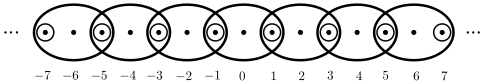
\includegraphics{Digital_line}}
\caption{The digital line topology.}
\label{F:Digital_line}
\end{center}
\end{figure}

In this exercise we explore the collection $\B = \{B(n)\}$. 

\ba
\item Show that the collection $\B = \{B(n)\}$ is a basis for a topology on $\Z$. (The resulting topology is called the \emph{digital line topology}\index{digital line topology} $\tau_{dl}$.\footnote{This digital line topology has applications in digital processing -- see \emph{Introduction to Topology: Pure and Applied} by Colin Adams and Robert Franzosa , Pearson Education, Inc., 2008,  Sections 1.4 and 11.3. The set $\Z$ with the digital line topology is called the \emph{digital line}.} (The digital line models a one-dimensional array of pixels, where the even integers are the pixels and the odd integers are boundaries between the pixels. Information about the \emph{digital plane} can be found in Section \ref{sec:Product_topology}.)


\item Determine which of the following sets are open in the digital line topology:
	\begin{enumerate}[i.]
	\item $\{0\}$
	\item $\{1\}$
	\item $\{0, 2\}$
	\item $\{1, 2, 3, 4, 5\}$
	\item $\Z^+$
	\item The set of odd integers.
	 \end{enumerate}
	 
\ea

\begin{comment}

\ExerciseSolution

\ba

\item Let $m \in \Z$ and suppose that $m$ is in $B_1 \cap B_2$ for some $B_1$ and $B_2$ in $\B$. Consider the case where $m$ is odd. Then $m \in B(m)$, $m \in B(m+1)$ and $m \in B(m-1)$. So $B_1$ and $B_2$ are one of $B(m)$, $B(m-1)$, and $B(m+1)$. In any case, $B(m)$ is then a subset of $B_1 \cap B_2$. 

Now consider the case where $m$ is even. Then $m \in B_(m)$ only. So $B_1 = B_2 = B(m)$, and $B(m) \subseteq B_1 \cap B_2$. We conclude that $\B$ is a basis for a topology on $\Z$. 

\item 	
	\begin{enumerate}[i.]
	\item The smallest open set that contains $0$ is $B(0) = \{-1,0,1\}$. So $\{0\}$ is not an open set. 
	\item Since $\{1\} = B(1)$, it follows that $\{1\}$ is an open set. 
	\item Any basis set that contains $0$ or $2$, also contains $1$. So $\{0, 2\}$ is not an open set. 
	\item Since $\{1, 2, 3, 4, 5\} = B(2) \cup B(4)$, it follows that the set $\{1, 2, 3, 4, 5\}$ is open.
	\item We can write $\Z^+$ as $\bigcup_{n \in \Z^+} B(n)$, so $\Z^+$ is an open set. 
	\item The set of odd integers can be written as $\bigcup_{n \text{ odd}} B(n)$, so the set of odd integers is an open set. 
	
	 \end{enumerate}

\ea

\end{comment}

\item \label{ex:TS_Zariski} Let $n$ be a positive integer and let $\mathcal{P}_n$ be the collection of all polynomials in $n$ real variables $x_1$, $x_2$, $\ldots$, $x_n$.  As a specific example, the polynomial 
\[f(x_1,x_2,x_3) = 2x_1x_3 + 5x_1x_2^2x_3^4 - x_2 + 10x_1^5x_3\]
is in $\mathcal{P}_3$. If $f(x_1, x_2, \ldots, x_n)$ is in $\mathcal{P}_n$, let $Z(f)$ be the set of zeros of the polynomial $f$. That is, 
\[Z(f) = \{(x_1, x_2, \ldots, x_n) \mid f(x_1,x_2, \ldots, x_n) = 0\}.\]
Note that $Z(f)$ is a subset of $\R^n$. For example, if $n=2$ and $f(x_1,x_2) = x_1^2 - x_2$ then $Z(f)$ is the set of ordered pairs in $\R^2$ satisfying $x_1^2-x_2 = 0$, or $x_2 = x_1^2$. This is the graph of the parabola $y=x^2$ in the plane. 

\ba

\item Describe $Z(f)$ in $\R^2$ if $f(x_1,x_2) = x_1^2 - 1$. 

\item If $E$ is a set of polynomials in $\mathcal{P}_n$, we let $Z(E) = \bigcap_{f \in E} Z(f)$ be the set of common zeros of all of the polynomials in $E$. Describe $Z(E)$ if $E = \{x_1+x_2+x_3, x_1-x_2-x_3, 3x_1+x_2+x_3\}$ in $\R^3$. 

%\item Let $E$ be a set of polynomials in $\mathcal{P}_n$. Prove or disprove $Z(E) = \bigcap_{f \in E} Z(f)$. 

\item Let $\mathcal{B}$ be the set of complements of the sets $Z(f)$ for $f \in \mathcal{P}_n$. Show that $\mathcal{B}$ is a basis for a topology on $\R^n$. The resulting topology is called the \emph{Zariski}\index{Zariski topology}\index{topology!Zariski} topology.

\item Is the set $S = \{(x_1,x_2) \in \R^2 \mid x_1 = 0 \text{ or } x_2 = 0\}$ an open set in $\R^2$ with the Zariski topology? Explain.  

\item Explain why the Zariski topology when $n=1$ is just the cofinite topology on $\R$. That is, show that every set that is open in the cofinite topology is open in the Zariski topology and that every set that is open in the Zaariski topology is open in the cofinite topology. 


\ea
 
\begin{comment}

\ExerciseSolution
 
\ba

 \item The zeros of the polynomial $f(x_1,x_2) = x_1^2 - 1$ occur when $x_1 = 1$ or $x_1 = -1$, while $x_2$ can take on any value. So $Z(x_1^2-1)$ is the union of the two lines $x=-1$ and $x=1$ in $\R^2$. 
 
 \item A little linear algebra shows that the reduced row echelon form of the matrix $\left[ \begin{array}{crr} 1&1&1 \\ 1&-1&-1 \\ 3&1&1 \end{array} \right]$ is $\left[ \begin{array}{ccc} 1&0&0 \\ 0&1&1 \\ 0&0&0 \end{array} \right]$. So $Z(E) = \{ (x_1,x_2,x_3) \mid x_2 = -x_3\}$ in $\R^3$. 

%\item Let $a \in Z(E)$ and let $f \in E$. Then $f(a) = 0$ and $a \in Z(f)$. It follows that $a \in \bigcap_{f \in E} Z(f)$. Now let $a \in \bigcap_{f \in E} Z(f)$. Then $f(a) = 0$ for every $f \in E$. Thus, $a \in Z(E)$. We conclude that $Z(E) = \bigcap_{f \in E} Z(f)$.

\item Let $a = (a_1,a_2,\ldots, a_n)$ be in $\R^n$. Let $f(x_1,x_2, \ldots, x_n) = 1$. Since $f(a) \neq 0$, $a \notin Z(f)$ and so $a \in \R^n \setminus Z(f)$. 

Now suppose that $B_1$ and $B_2$ are in $\mathcal{B}$ and $a \in B_1 \cap B_2$. Then $B_1 = \R^n \setminus Z(f_1)$ and $B_2 = \R^n \setminus Z(f_2)$ for some polynomials $f_1$ and $f_2$. Since $a \in B_1$, it follows that $f_1(a) \neq 0$. Similarly, since $a \in B_2$ we know that $f_2(a) \neq 0$. So $(f_1f_2)(a) = f_1(a)f_2(a) \neq 0$ and $a \notin Z(f_1f_2)$ and $a \in \R^n \setminus Z(f_1f_2)$. Thus, $\mathcal{B}$ is a basis for a topology on $\R^n$. 

\item The set $\{(0,x_2) \mid x_2 \in \R\}$ is $Z(x_1)$ while the set $\{(x_1,0) \mid x_1 \in \R\}$ is $Z(x_2)$. Now $B_1 = \R^2 \setminus Z(x_1)$ and $B_2 = \R^2 \setminus Z(x_2)$ are both open sets, and $S = B_1 \cap B_1$. As a finite intersection of open sets, we conclude that $S$ is an open set. 

\item Every polynomial in $\mathcal{P}_1$ has the form $ax+b$ where $a, b \in \R$. If $a \neq 0$, the only way $ax+b$ can have zeros is if $b = 0$. If $a \neq 0$ then the zeros of $ax+b$ are the same as the zeros of $x + \frac{b}{a}$. From this perspective we can just consider monic polynomials in $\mathcal{P}_1$. 

Let $O$ be an open set in $\R$ with the cofinite topology. Then $\R \setminus O$ is finite. Let $\R \setminus O = \{a_1, a_2, \ldots, a_k\}$. Let $f(x) = (x-a_1)(x-a_2) \cdots (x-a_k)$. Then $Z(f) = \R \setminus O$ and $\R \setminus Z(f) = O$. Thus, every set that is open in the cofinite topology is open in the Zariski topology.

To show that every open set in the Zariski topology is open in the cofinite topology, it suffices to show that this is true for the basis elements in the Zariski topology. Let $B = \R \setminus Z(f)$ be an open basis element in the Zariski topology, where $f$ is some polynomial in $\mathcal{P}_n$. Since $f$ can have only finitely many roots, the set $\R \setminus B = Z(f)$ is finite, and so $B$ is open in the cofinite topology. We conclude that the Zariski topology and cofinite topology are the same when $n =1$. Note that argument will not be valid when $n \geq 2$ because $Z(f)$ can be an infinite set.   

\ea

\end{comment}

\item For each of the following, answer true if the statement is always true. If the statement is only sometimes true or never true, answer false and provide a concrete example to illustrate that the statement is false. If a statement is true, explain why. 
	\ba
	\item The set $\{\emptyset, \{a,b\}, \{a,b,d,f\}, \{d,f\},X\}$ is a topology on the set $X = \{a,b,c,d,e,f\}$.

	\item  The set $\Z$ is an open subset of $\R$ using the finite complement topology $\tau_{FC}$ on $\R$.

	\item The set $\mathcal{B} = \{\{b\},\{c\}, \{a,b\}, \{b,c,d\}\}$ is a basis for the topology $\tau$ on the set $X = \{a,b,c,d\}$, where 
\[\tau = \{\emptyset, \{b\}, \{c\}, \{a,b\}, \{b,c\}, \{a,b,c\}, \{b,c,d\}, X\}.\]

	\item Let $X$ be a nonempty set. If $\tau$ is the discrete topology, then the topological set $(X,\tau)$ is metrizable.  

	\item The point $b$ is an interior point of the subset $A = \{a,b,d\}$ in the topological space $(X,\tau)$, where $X = \{a,b,c,d\}$ and 
\[\tau = \{\emptyset, \{a\}, \{a,b\}, \{c\}, \{d\}, \{c,d\}, \{a,c,d\}, \{a,c\}, \{a,d\}, \{a,b,c,\}, \{a,b,d\}, X\}.\]

	\item If $\tau_1$ and $\tau_2$ are topologies on a space $X$, then $\tau_1 \cup \tau_2$ is also a topology on $X$.  
	
	\item If $\tau_1$ and $\tau_2$ are topologies on a space $X$, then $\tau_1 \cap \tau_2$ is also a topology on $X$.
	
	\ea

\begin{comment}

\ExerciseSolution

\ba

	\item This statement is true. By definition, $\tau$ contains $\emptyset$ and $X$. The unions of the non-trivial sets in $\tau$ are 
	\[\{a,b\} \cup \{a,b,d,f\} = \{a,b,d,f\}, \{d,f\} \cup \{a,b,d,f\} = \{a,b,d,f\}, \text{ and } \{a,b\} \cup \{d,f\} = \{a,b,d,f\},\]
	and these unions are all in $\tau$. It is also the case that the intersections 
	\[\{a,b\} \cap \{a,b,d,f\} = \{a,b\}, \{d,f\} \cap \{a,b,d,f\} = \{d,f\}, \text{ and } \{a,b\} \cap \{d,f\} = \emptyset,\]
	of the non-trivial sets in $\tau$ are also in $\tau$. 
	
	\item  This statement is false since $\R \setminus \Z$ is not finite. 
	
	\item This statement is true. By inspection we can see that every element in $X$ is an element of some set in $\mathcal{B}$. Letting $B_1 = \{b\}$, $B_2 = \{c\}$, $B_3 = \{a,b\}$, and $B_4 = \{b,c,d\}$, we have that the intersections of the sets in $\mathcal{B}$ are 
	\begin{align*}
	B_1 \cap B_2 &= B_2 \cap B_3 = \emptyset, \\
	B_1 \cap B_i &= \{b\}, \text{ where } 3 \leq i \leq 4, \\
	B_2 \cap B_4 &= \{c\}, \text{ and } \\
	B_3 \cap B_4 &= \{b\}.
	\end{align*}
The only elements in $X$ that are in $B_i \cap B_j$ for some $i$ and $j$ are $b$ and $c$. But then either $B_1$ or $B_2$ is a subset of $B_i \cap B_j$. We conclude that $\mathcal{B}$ is a basis for $\tau$. 

	\item This statement is true since the topological space $(X,\tau)$ has the same open sets as the $(X, d)$, where $d$ is the discrete metric. 
	
	\item This statement is true since $\{a,b\}$ is an open set that contains $b$ and is also a subset of $A$. 

	\item This statement is false. Let $X = \{a,b,c\}$ with $\tau_1 = \{\emptyset, \{a\}, X\}$ and $\tau_2 =  \{\emptyset, \{b\}, X\}$. Then $\tau_1 \cup \tau_2 = \{\emptyset, \{a\}, \{b\}, X\}$. But $\{a\} \cup \{b\}$ is not in $\tau_1 \cup \tau_2$. 
		
	\item This statement is true. By definition, both $\emptyset$ and $X$ are in $\tau_1 \cap \tau_2$. Let $\{O_{\alpha}\}$ be a collection of sets in $\tau_1 \cap \tau_2$ for $\alpha$ in some indexing set $I$. Then each $O_{\alpha}$ is in $\tau_1$ and $\tau_2$, which means that $\bigcup_{\alpha \in I} O_{\alpha}$ is also in $\tau_1$ and $\tau_2$. Thus, $\bigcup_{\alpha \in I} O_{\alpha}$ is in $\tau_1 \cap \tau_2$. Similarly, if $I$ is finite, then $\bigcap_{\alpha \in I} O_{\alpha}$ is in $\tau_1$ and $\tau_2$, which means $\bigcap_{\alpha \in I} O_{\alpha}$ is in $\tau_1 \cap \tau_2$.
	
\ea

\end{comment}

\ee
